\let\negmedspace\undefined
\let\negthickspace\undefined
\documentclass[journal,12pt,onecolumn]{IEEEtran}
\usepackage{cite}
\usepackage{amsmath,amssymb,amsfonts,amsthm}
\usepackage{algorithmic}
\usepackage{graphicx}
\graphicspath{{Figs/}}
\usepackage{textcomp}
\usepackage{xcolor}
\usepackage{txfonts}
\usepackage{listings}
\usepackage{enumitem}
\usepackage{mathtools}
\usepackage{gensymb}
\usepackage{comment}
\usepackage{caption}
\usepackage[breaklinks=true]{hyperref}
\usepackage{tkz-euclide} 
\usepackage{listings}
\usepackage{gvv}                                        
%\def\inputGnumericTable{}                                 
\usepackage[latin1]{inputenc}     
\usepackage{xparse}
\usepackage{color}                                            
\usepackage{array}                                            
\usepackage{longtable}                                       
\usepackage{calc}                                             
\usepackage{multirow}
\usepackage{multicol}
\usepackage{hhline}                                           
\usepackage{ifthen}                                           
\usepackage{lscape}
\usepackage{tabularx}
\usepackage{array}
\usepackage{float}
%\newtheorem{theorem}{Theorem}[section]
%\newtheorem{theorem}{Theorem}[section]
%\newtheorem{problem}{Problem}
%\newtheorem{proposition}{Proposition}[section]
%\newtheorem{lemma}{Lemma}[section]
%\newtheorem{corollary}[theorem]{Corollary}
%\newtheorem{example}{Example}[section]
%\newtheorem{definition}[problem]{Definition}

\begin{document}


\title{3.2.13}
\author{AI25BTECH11002 - Ayush Sunil Labhade}
{\let\newpage\relax\maketitle}

\textbf{Question}:\newline

Draw a triangle ABC in which AB=5cm, BC=6cm and $\angle ABC=60^\circ$.
\newline
\textbf{Solution:}\newline
The triangle can be plotted by taking $B = (0,0)$ and $A = (5,0)$.
Therefore, $C$ will be:
\[
C = (6\cos 60^\circ,\;6\sin 60^\circ)
\]

Thus, the points are:
\begin{table}[H]
    \centering
    \begin{tabular}{|c|c|}
\hline
Point & Vector \\
\hline
$\vec{A}$ & $\myvec{5 \\ 0}$ \\
\hline
$\vec{B}$ & $\myvec{0 \\ 0}$ \\
\hline
	$\vec{C}$ & $\myvec{6\cos(60^\circ) \\ 6\sin(60^\circ) }$ \\
\hline
\end{tabular}

    \caption{Points data}
    \label{tab:points}
\end{table}

Graph:
\begin{figure}[H]
    \centering
    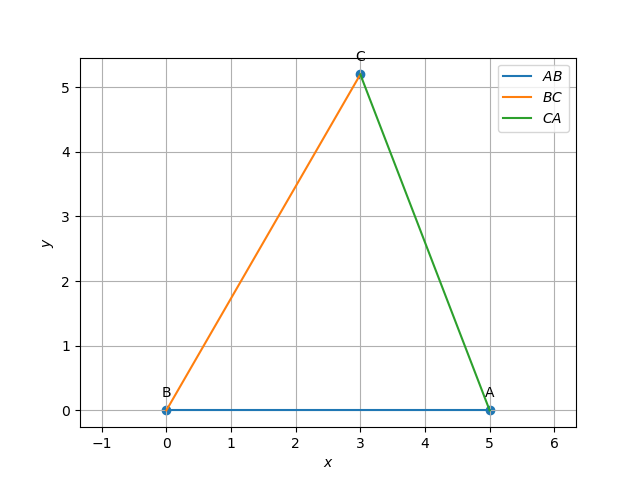
\includegraphics[scale=0.5]{plot}
    \caption{}
    \label{fig:plot}
\end{figure}
\end{document}
